\documentclass[conference]{IEEEtran}
\IEEEoverridecommandlockouts
% The preceding line is only needed to identify funding in the first footnote. If that is unneeded, please comment it out.
\usepackage{cite}
\usepackage{amsmath,amssymb,amsfonts}
\usepackage{algorithmic}
\usepackage{graphicx}
\usepackage{textcomp}
\usepackage{xcolor}
\def\BibTeX{{\rm B\kern-.05em{\sc i\kern-.025em b}\kern-.08em
    T\kern-.1667em\lower.7ex\hbox{E}\kern-.125emX}}
\begin{document}

\title{CENG435 Term Project 2\\
{\footnotesize \textsuperscript{*}UDP-based "Reliable Data Transfer" (RDT) protocol}
\thanks{}
}

\author{\IEEEauthorblockN{1\textsuperscript{st} Furkan TASBASI}
\IEEEauthorblockA{\textit{METU} \\
\textit{CENG}\\
Ankara, Turkey \\
}
\and
\IEEEauthorblockN{2\textsuperscript{nd} Batuhan BAT}
\IEEEauthorblockA{\textit{METU} \\
\textit{CENG}\\
Ankara, Turkey \\
}
}

\maketitle

\section{Design}
First of all, before code process we designed our TCP(Transmission Control Protocol) and UDP(User Datagram Protocol) server-client structures and also decided on our RDT(Reliable Data Transfer) and calculating checksum algorithm according to a data consisting of 100 bytes(characters). Source computer gets whole data from a file named "file.txt" 100 characters for each step. Then source creates a TCP connection to the broker and sends a data which compounds from 100 bytes to broker. Here source node has TCP client features. Then broker listens network via it's interface from source with TCP Server behavior. Whenever it takes a 100 bytes data, it starts to packetize it into 10 different packets by firstly adding index information of single integer character(this integer will later be converted to string to be able to add to end of the message packet to be sent) to end of each packet. After adding index information; to the end of every packet a single character is added as a checksum character which makes every packet sized of 12 character length(10 char's from message and + 1 int from helper index and + 1 char from checksum).
$\newline$

When calculating the checksum character at the end of each packet, we decided to choose an algorithm such that it will give unique results for each packet. So we decided to follow an approach where we find ASCII(American Standard Code for Information Interchange) equals of each of the ten characters in the broken message pieces and sum up all those ten ASCII equals and apply a modulo operation of 100(hundred) to get a unique integer between 0 and 99 for each broken message piece of 10 characters. Then this calculated checksum is added to the end of each packet to be sent which was 11 characters in length(10 for message and +1 for sequence number). So after adding checksum the messages to be sent becomes 12 characters in length.

After packetizing process, broker sends all packets to destination via routers with UDP client behavior. Routing from Broker to Router devices works according to a simple function named Dest$\_$Chose() which continuously does altering between two paths(the first path connects broker and destination through Router1, while the second path connects broker and destination through Router2). Router devices directly behaves as if a real router which connects two different subnets together. Whenever a router takes a packet, it sends it to destination device according to its kernel routing table which we have configured with kernel route commands. After all routing process, destination takes 120 bytes single data from network by listening its two different interfaces connected to Router1 and Router2 with UDP server behavior. Destination waits for 12 character long packets. Whenever the destination receives a packet with 12 character length, it firstly checks the last character which is the checksum value. If the checksum character of the received packet is exactly same with the checksum character calculated at the destination, then it means the related packet is received without any problems. Here, the destination distinguishes the relevant packet according to their indexes which is actually the sequence number. So destination now sends an ACK(positive acknowledgment) to the broker. So when the broker gets this ACK, the broker will mark its helper isAcked array's relevant element to a 1 meaning that the relevant packet is received by the destination successfully. If checksum character of the received packet does not fit with the calculated checksum at the destination, the destination sends a NACK(negative acknowledgment) to the broker. When the broker gets this NACK, the broker will mark its helper isAcked array's relevant element to a -1 meaning that the relevant packet is not received by the destination successfully. At the end, when the destination receives all the packets, it uses the index numbers of the packets and in this way, it sorts and organizes the received packets as a complete message of 100 characters in length. 

After sending a packet, broker waits for ACK or NACK packets for sent packet. Whenever it takes an ACK packet from destination, it then marks relevant index of isAcked array to prevent possible dublications in future for resending. Meanwhile, broker sets the ending time for the ACKed packet's into the Delay array that we marked the starting time of sending packet at the moment of sending process for a sending packet. With the help of Delay array we will have both start and end times for particular packets so we calculate delay times of packets via Delay array which consists of 10 elements each itself an array of 2 elements again(first float represents packet sending time information, second float represents packet arrival time information). If broker takes a NACK packet, it sends the relevant packet again. By the way, we update the DevRTT for all ACK and NACK packet incoming processes to get best time-out interval. In this project we applied a process same with the one in the textbook DevRTT calculations. If broker does not take any ACK or NACK packet for a particular packet sent before, it then marks the relevant index of TimeOut array to know which packets are needed to be re-sent because of time-out problem. As we choose to follow an approach like this, we have actually implemented a Selective Repeat Approach as a pipelined networking. Our RDT uses the following mechanisms: checksum, retransmission, ACK/NACK mechanism, sequence number(which is called as index number in our implementation) and buffering. 

While measuring the end-to-end delays, we have seen such non-synchronized devices as a timestamp, we have used NTP(network time protocol) comments to  synchronize all devices. We have used "time.nist.gov" servers for this purpose. Then, we have validated that there is no clock difference between devices. 

\section{Experiment}

While doing experiments, we have sent 100 different data containing 10 packet sets that each of them including 10(ten) packets and measured the average network delays as $17.8$ s, $17.9$ s, $3539.7$ s, $14.8$ s for $16.3$ s, $9739.5$ s, $12.9$ s, $14.3$ s $11.2$ s in relative order. After that, we have calculated standart deviations of each experiment sets then applied them to the formula with corresponding confidence interval values step by step for all experiments. While applying the formula, we have multiplied average values with Z value (which is 1.96 for $.95$ confidence interval), then multiplied the sub result with the value of standart deviation divided by square root of sample size which is 10 ($\sqrt{n}$ where n is 100). As a result we have found confidence intervals as $0.671377489444897$,
$1.11813567055961$,
$1316.34917831071$,
$0.180111570360646$,
$1.11277838464509$,
$2339.61686147321$,
$0.171616627011099$,
$0.132289917311268$, 
$0.755158379267408$ 
(in seconds) respectively for experiments in relative order.
Finally, we draw three graphs including these errors for all points.

\section*{Figures}
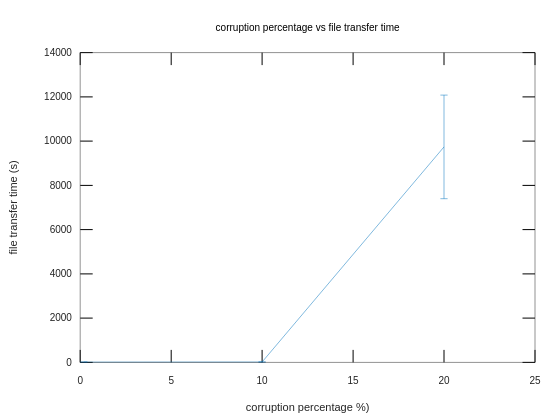
\includegraphics[height=200pt]{corruption.png}

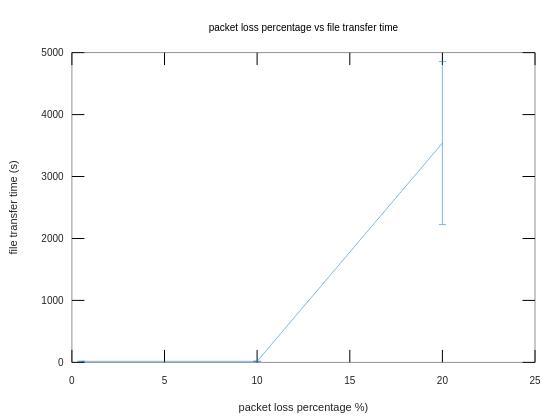
\includegraphics[height=200pt]{packloss.png}

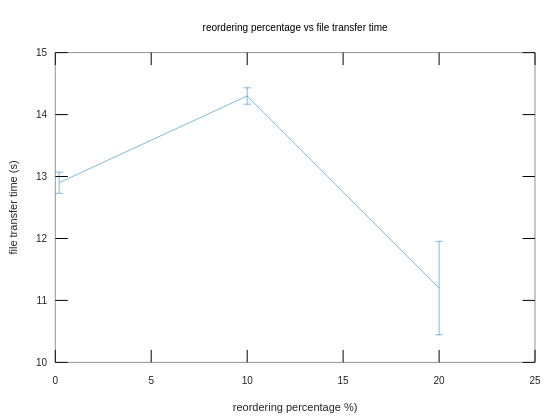
\includegraphics[height=200pt]{reordering.png}

$\newline$
$\newline$
$\newline$

As we can recognize from the first graph given above that there is a linear correspondence between file transfer time and corruption percentage after 10 percentage that means because of corruption in network, our RDT mechanism does retransmission which causes increase in time to send all data. If we analyze the second graph which shows the linear correspondence between file transfer time and packet loss rate. Our RDT does retransmission because of timeout which is calculated up to current DevRTT value. Since , DevRTT value approaches to better timeout values in real time network traffic, it sends lost packets in smaller time in comparison with corrupted packet case. Lastly, if we look at the third graph which shows reordering in network and its relationship with file transfer time, file transfer time increases linearly up to 10 percentage of reordering and then decreases linearly after this point which shows our worst case of file transfer time is reordering of 1 out of 10 packets that we have found out in our experiments.

\section*{Notification}
All homework processes(design, writing the report, code implementation, commenting codes, configurations and graphs) are done together with both group members and GoogleDrive is used for version control for all homework.
$\newline$

Router configurations are named as router$\_$configurations.ods file which is given in homework submission folder.  

\end{document}